% !TEX encoding = UTF-8 Unicode
% !TEX TS-program = pdflatex

\documentclass{article}
	\usepackage{tikz}
	\usepackage{listings}
\begin{document}

	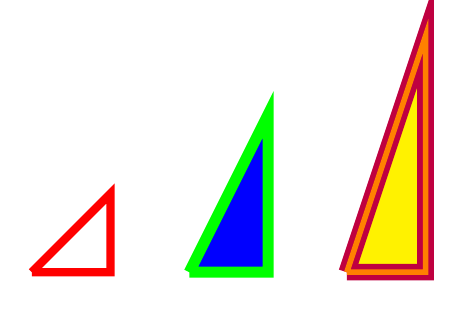
\begin{tikzpicture}
		\draw [red, line width=3pt] (0,0)--(1,0)--(1,1)--(0,0) ;
		\filldraw[fill=blue, draw=green, line width=4](2,0)--(3,0)--(3,2)--(2,0);
		\filldraw[fill=yellow,draw=purple, line width=6](4,0)--(5,0)--(5,3)--(4,0);
		\draw    [            draw=orange, line width=2](4,0)--(5,0)--(5,3)--(4,0);
	\end{tikzpicture}

\lstset{language=[latex]tex,tabsize=4}
\lstset{moretexcs={draw,filldraw}}
\begin{lstlisting}
% !TEX encoding = UTF-8 Unicode
% !TEX TS-program = pdflatex
\documentclass{article}
	\usepackage{tikz}
\begin{document}
	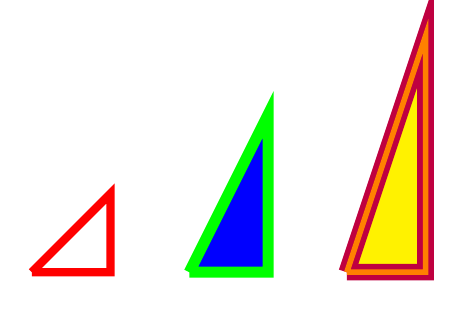
\begin{tikzpicture}
		\draw [red, line width=3pt] (0,0)--(1,0)--(1,1)--(0,0) ;
		\filldraw[fill=blue, draw=green, line width=4]
			(2,0)--(3,0)--(3,2)--(2,0);
		\newcommand\thintriangle{(4,0)--(5,0)--(5,3)--(4,0)}
		\filldraw[fill=yellow, draw=purple, line width=6] \thintriangle ;
		\draw    [             draw=orange, line width=2] \thintriangle ;
	\end{tikzpicture}
\end{document}
\end{lstlisting}

\end{document}